\documentclass[9pt, conference]{IEEEtran}
\IEEEoverridecommandlockouts

\usepackage{amsmath,amsfonts,graphicx}
\usepackage{amssymb,textcomp,mathtools}
\usepackage{bm,upgreek,algorithm,hyperref}
\usepackage{multirow,booktabs,hhline,array}
\usepackage{cite,url,makecell,setspace}
\usepackage{xcolor}
\pdfoutput=1

\def\thline{\noalign{\hrule height 1.0pt}}
\def\tthline{\noalign{\hrule height 1.4pt}}
\DeclareMathOperator*{\argmin}{argmin}
\DeclareMathOperator*{\argmax}{argmax}

\renewcommand{\vec}[1]{\bm{\mathrm{#1}}}
\def\x{{\mathbf x}}
\def\L{{\cal L}}

\title{Apollo: Band-sequence Modeling for High-Quality Audio Restoration}

\author{\IEEEauthorblockN{Kai~Li$^{\spadesuit,\clubsuit,*}$, Yi Luo$^{\clubsuit,*}$\\}
\IEEEauthorblockA{$^\spadesuit$Department of Computer Science and Technology, Tsinghua University, Beijing, China \\
$^\clubsuit$Tencent AI Lab, Shenzhen, China \\
tsinghua.kaili@gmail.com, oulyluo@tencent.com}
\thanks{$*$ The work was done while Yi Luo was at Tencent AI Lab and Kai Li was an intern there.}
}

\begin{document}
\maketitle

\begin{abstract}
Scaling Transformers to longer sequence lengths has been a major problem in the
last several years, promising to improve performance in language modeling and
high-resolution image understanding, as well as to unlock new applications in
code, audio, and video generation.
The attention layer is the main bottleneck in scaling to longer sequences, as
its runtime and memory increase quadratically in the sequence length.
\sysnameone~\citep{dao2022flashattention} exploits the asymmetric GPU memory
hierarchy to bring significant memory saving (linear instead of quadratic) and
runtime speedup (2-4$\times$ compared to optimized baselines), with no approximation.
However, \sysnameone is still not nearly as fast as optimized matrix-multiply
(GEMM) operations, reaching only 25-40\% of the theoretical maximum FLOPs/s.
We observe that the inefficiency is due to suboptimal work partitioning between
different thread blocks and warps on the GPU, causing either low-occupancy or
unnecessary shared memory reads/writes.
We propose \sysname, with better work partitioning to address these issues.
In particular, we (1) tweak the algorithm to reduce the number of non-matmul
FLOPs (2) parallelize the attention computation, even for a single head, across
different thread blocks to increase occupancy, and (3) within each thread block,
distribute the work between warps to reduce communication through shared memory.
These yield around 2$\times$ speedup compared to \sysnameone, reaching 50-73\% of the
theoretical maximum FLOPs/s on A100 and getting close to the efficiency of GEMM
operations.
We empirically validate that when used end-to-end to train GPT-style models,
\sysname reaches training speed of up to 225 TFLOPs/s per A100 GPU (72\% model
FLOPs utilization).\footnote{\sysname
  is available at \url{https://github.com/Dao-AILab/flash-attention}}

% models with up to 2$\times$ longer sequence length compared to \sysnameone, in the
% same amount of time, leading to better downstream performance.\footnote{\sysname
%   is available at \url{https://github.com/Dao-AILab/flash-attention}}

\end{abstract}
\begin{IEEEkeywords}
Audio restoration, audio superresolution, bandwidth extension, generative adversarial network 
\end{IEEEkeywords}
\section{Introduction}
\label{sec:introduction}
\section{Introduction}
Despite the well-recognized importance of training data in advancing the capabilities of large language models (LLMs)~\cite{brown2020language,kaplan2020scaling,Razeghi2022ImpactOP}, there is no agreed-upon mechanisms for crediting or compensating data providers. As LLMs are increasingly integrated into our society and economy, the absence of such mechanisms has aggravated a tension between data and model providers, exemplified by recent legal challenges involving major tech companies~\cite{jlversusalphabet,metz2022lawsuit}. In this atmosphere, data valuation, which quantifies the contribution of each training data to the model output, has been discussed as a potential technical solution for tackling these societal issues~\cite{fernandez2023data,ghorbani2019data,huang2023citation,jia2019towards,worledge2023unifying,zhao2023addressing}. 

At a high level, most data valuation algorithms interpret the model output as a coalition of its training data, and evaluate the contribution of each example based on its influence on the model output when included or excluded from the training dataset~\cite{ghorbani2019data,ilyas2022datamodels,koh2017understanding,kwon2021beta}. If an inclusion of a specific training example consistently improves model performance, high value can be assigned to this example for its contribution. However, applying existing data valuation methods to recent LLMs and their vast training datasets has faced significant scalability challenges to date. For instance, sampling-based methods, such as the Shapley value~\cite{ghorbani2019data,kwon2021beta} or Datamodels~\cite{ilyas2022datamodels}, require retraining the model multiple times with varied combinations of data subsets to directly model the effect of in/excluding each data. Unfortunately, such repeated retraining is hardly affordable even for small models, let alone LLMs. To overcome this issue, gradient-based methods, including influence functions~\cite{koh2017understanding,park2023trak}, approximate the effect of data in/exclusion on the model output using gradient information without costly retraining. Even so, scaling gradient-based methods to LLMs is hindered by prohibitive compute and memory costs originating in the high-dimensional nature of the gradient.

Consequently, the main objective of this work is to bridge the gap in scaling existing data valuation methods to recent LLMs and their vast training datasets. Toward this goal, we focus on influence functions \cite{koh2017understanding,park2023trak}, a representative gradient-based data valuation method, and significantly improve its scalability with an efficient gradient projection algorithm. We visualize the proposed data valuation system in Figure~\ref{fig:diagram}, and detail our technical contributions below:

\begin{figure}
    \centering
    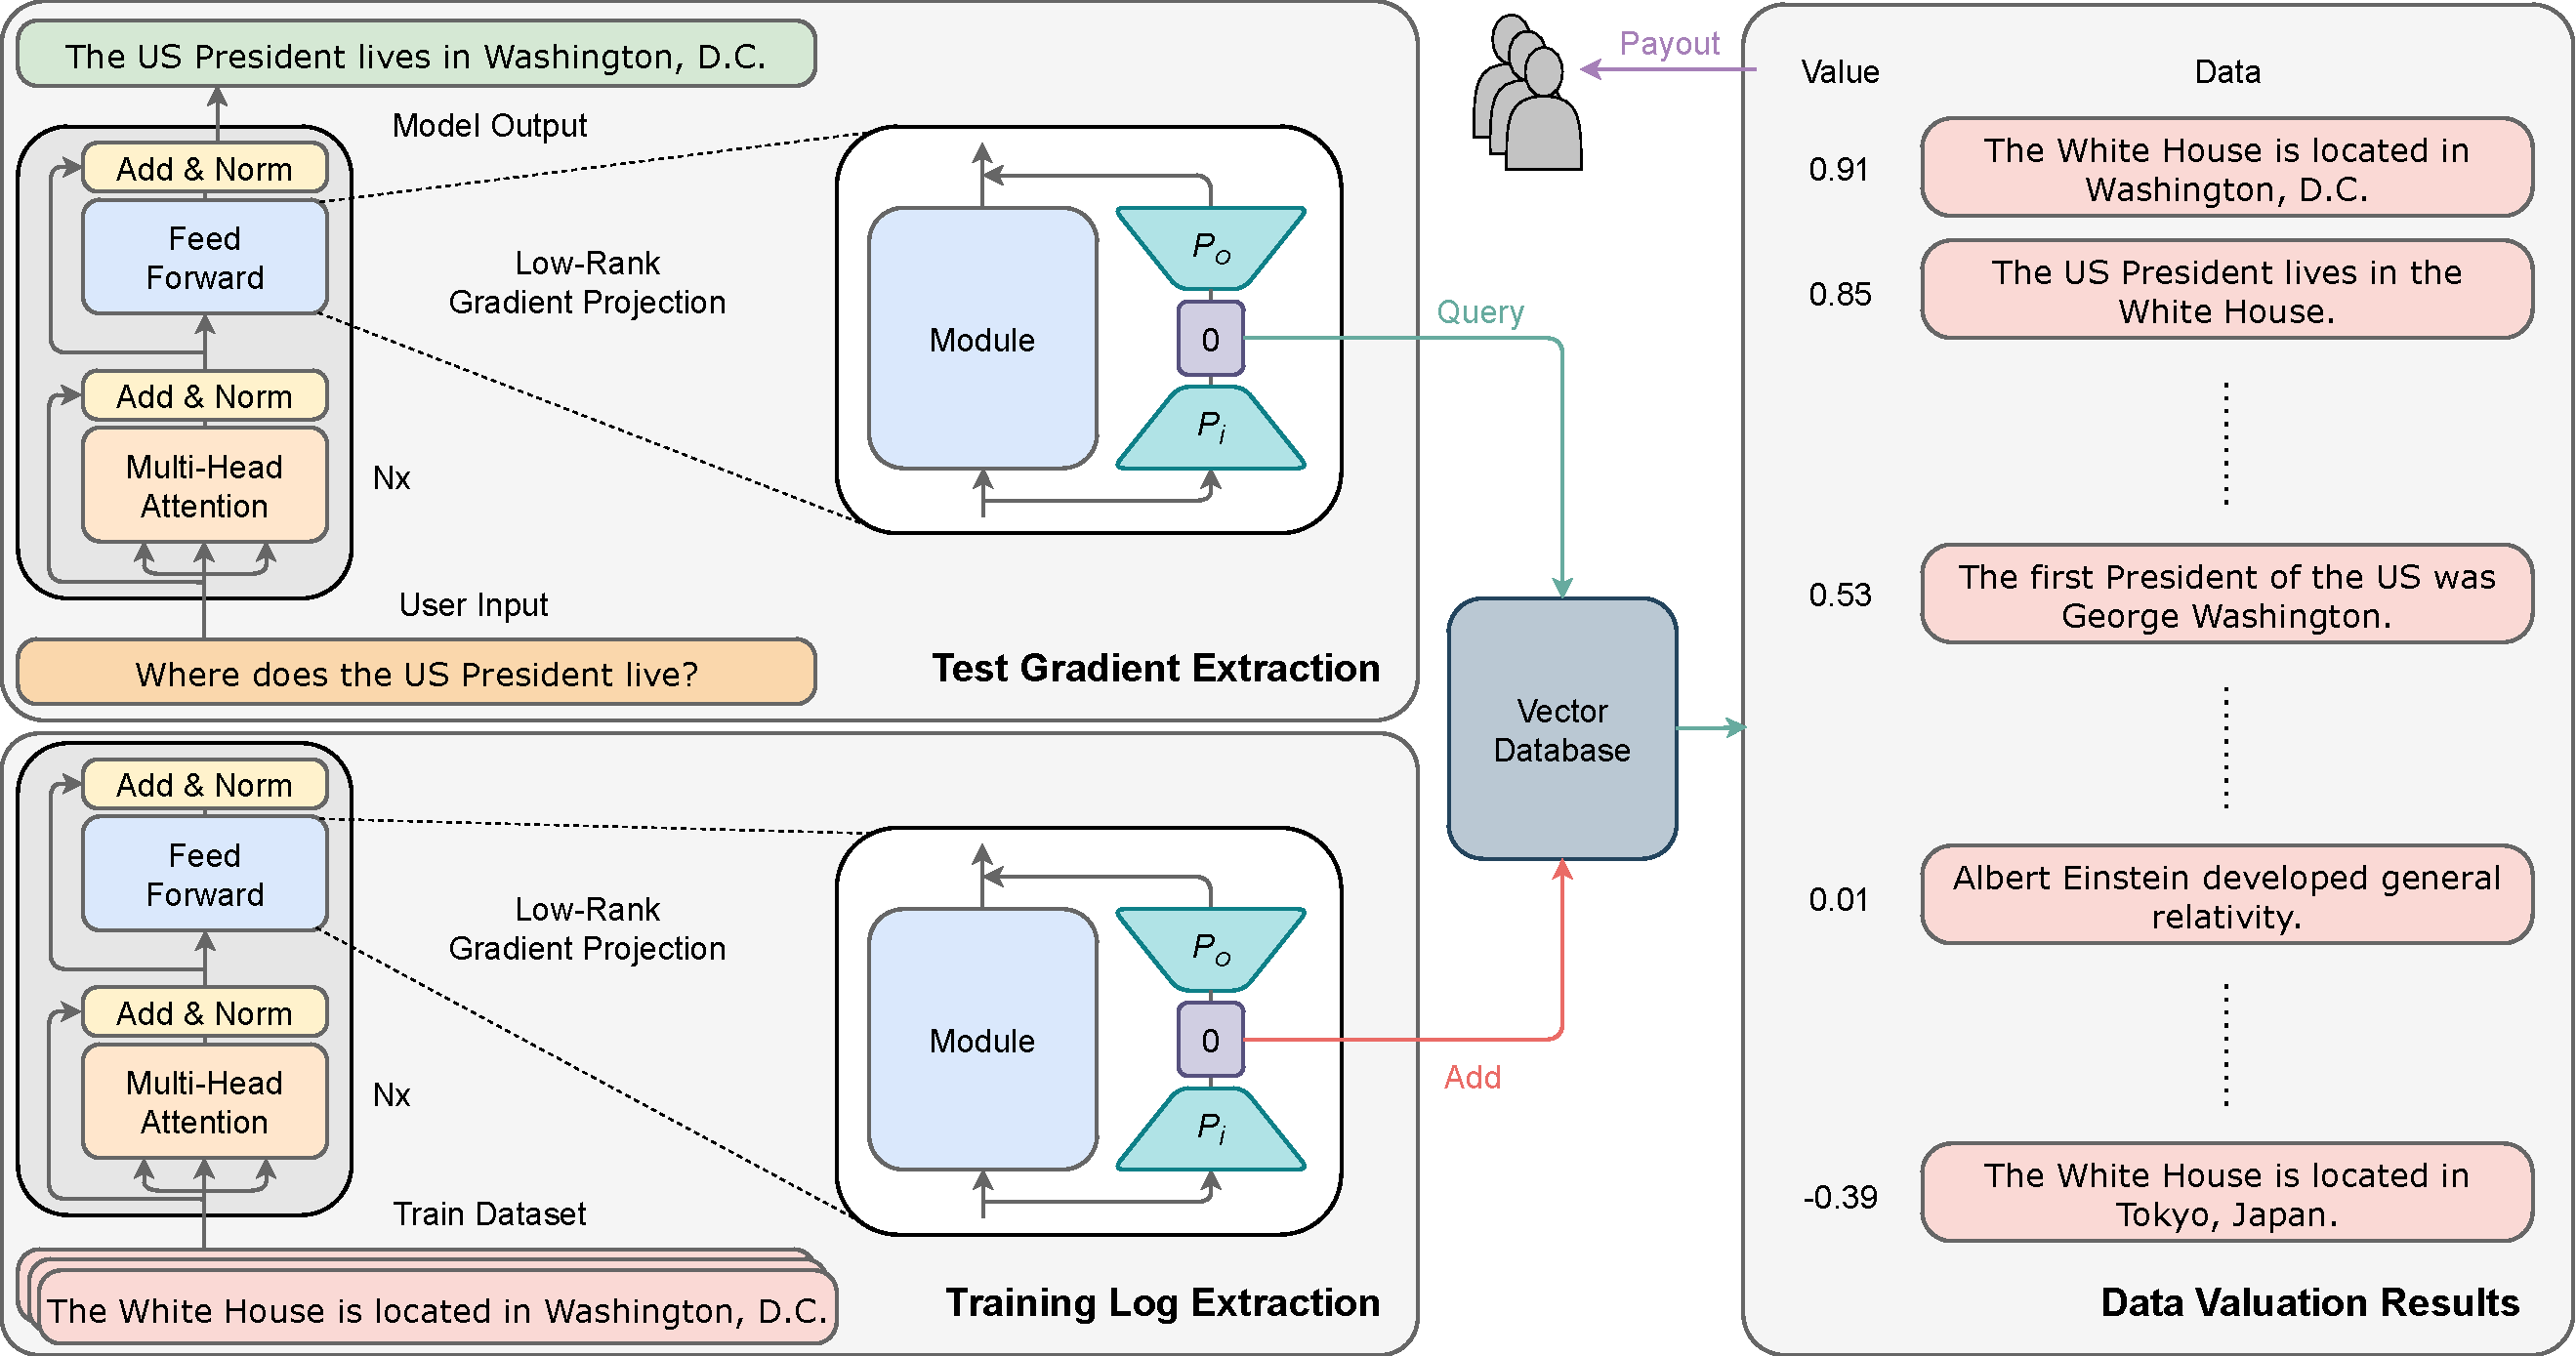
\includegraphics[width=0.94\textwidth]{figures/diagram_v7.pdf}
    \vskip -4pt
    \caption{Data valuation system architecture. \textbf{(Left Bottom)} We first extract the Hessian and gradients for all training data using efficient gradient projection \method\ and store them in a database. \textbf{(Left Top)} At test time, we similarly extract gradients and query the database. \textbf{(Right)} The database returns similarity scores with respect to training examples that can be used for data valuation/attribution.}
    \label{fig:diagram}
\end{figure}

\begin{itemize}[leftmargin=*,topsep=-2pt]
    \item Employing gradient structures in backpropagation, we develop a novel \textbf{lo}w-rank \textbf{gra}dient projection algorithm \method\ that improves space \& time complexity of gradient projection, a major scalability bottleneck in prior work~\cite{park2023trak,schioppa2022scaling}, from $O(nk)$ to $O(\sqrt{nk})$ where $n$ and $k$ are model and projection dimensions. Furthermore, \method\ directly computes projected gradients without materializing full gradients, enabling low GPU memory and high GPU utilization for improved efficiency. Lastly, we show that \method\ can be easily implemented with small add-on layers, similarly to LoRA~\cite{hu2021lora}.
    \item By interpreting a damping term in influence functions as a spectral gradient sparsification mechanism, we (1) offer a theoretical motivation of gradient projection approaches to influence functions and (2) derive a specialized PCA initialization scheme for \method.
    \item We introduce software named \software\ that (1) makes it \textit{simple} to convert existing training code into data valuation code, (2) is \textit{compatible} with various scalability tools and features in the LLM ecosystem, and (3) is \textit{extensible} to implement other data valuation or interpretability algorithms.
    \item In our data valuation experiments, \method\ demonstrates competitive accuracy against more costly baselines, while showing up to 6,500$\times$ increase in throughput and 5$\times$ reduction in GPU memory, when applied to Llama3-8B-Instruct~\cite{llama3modelcard} and the 1B-token dataset, compared to EKFAC influence \cite{grosse2023studying}, the state-of-the-art and only runnable baseline at this scale. We also observe that most valuable data identified by \method\ generally share qualitative similarities with the queried LLM output.
\end{itemize}

\section{Apollo}
\label{sec:model}
\begin{figure}[h]
\begin{center}
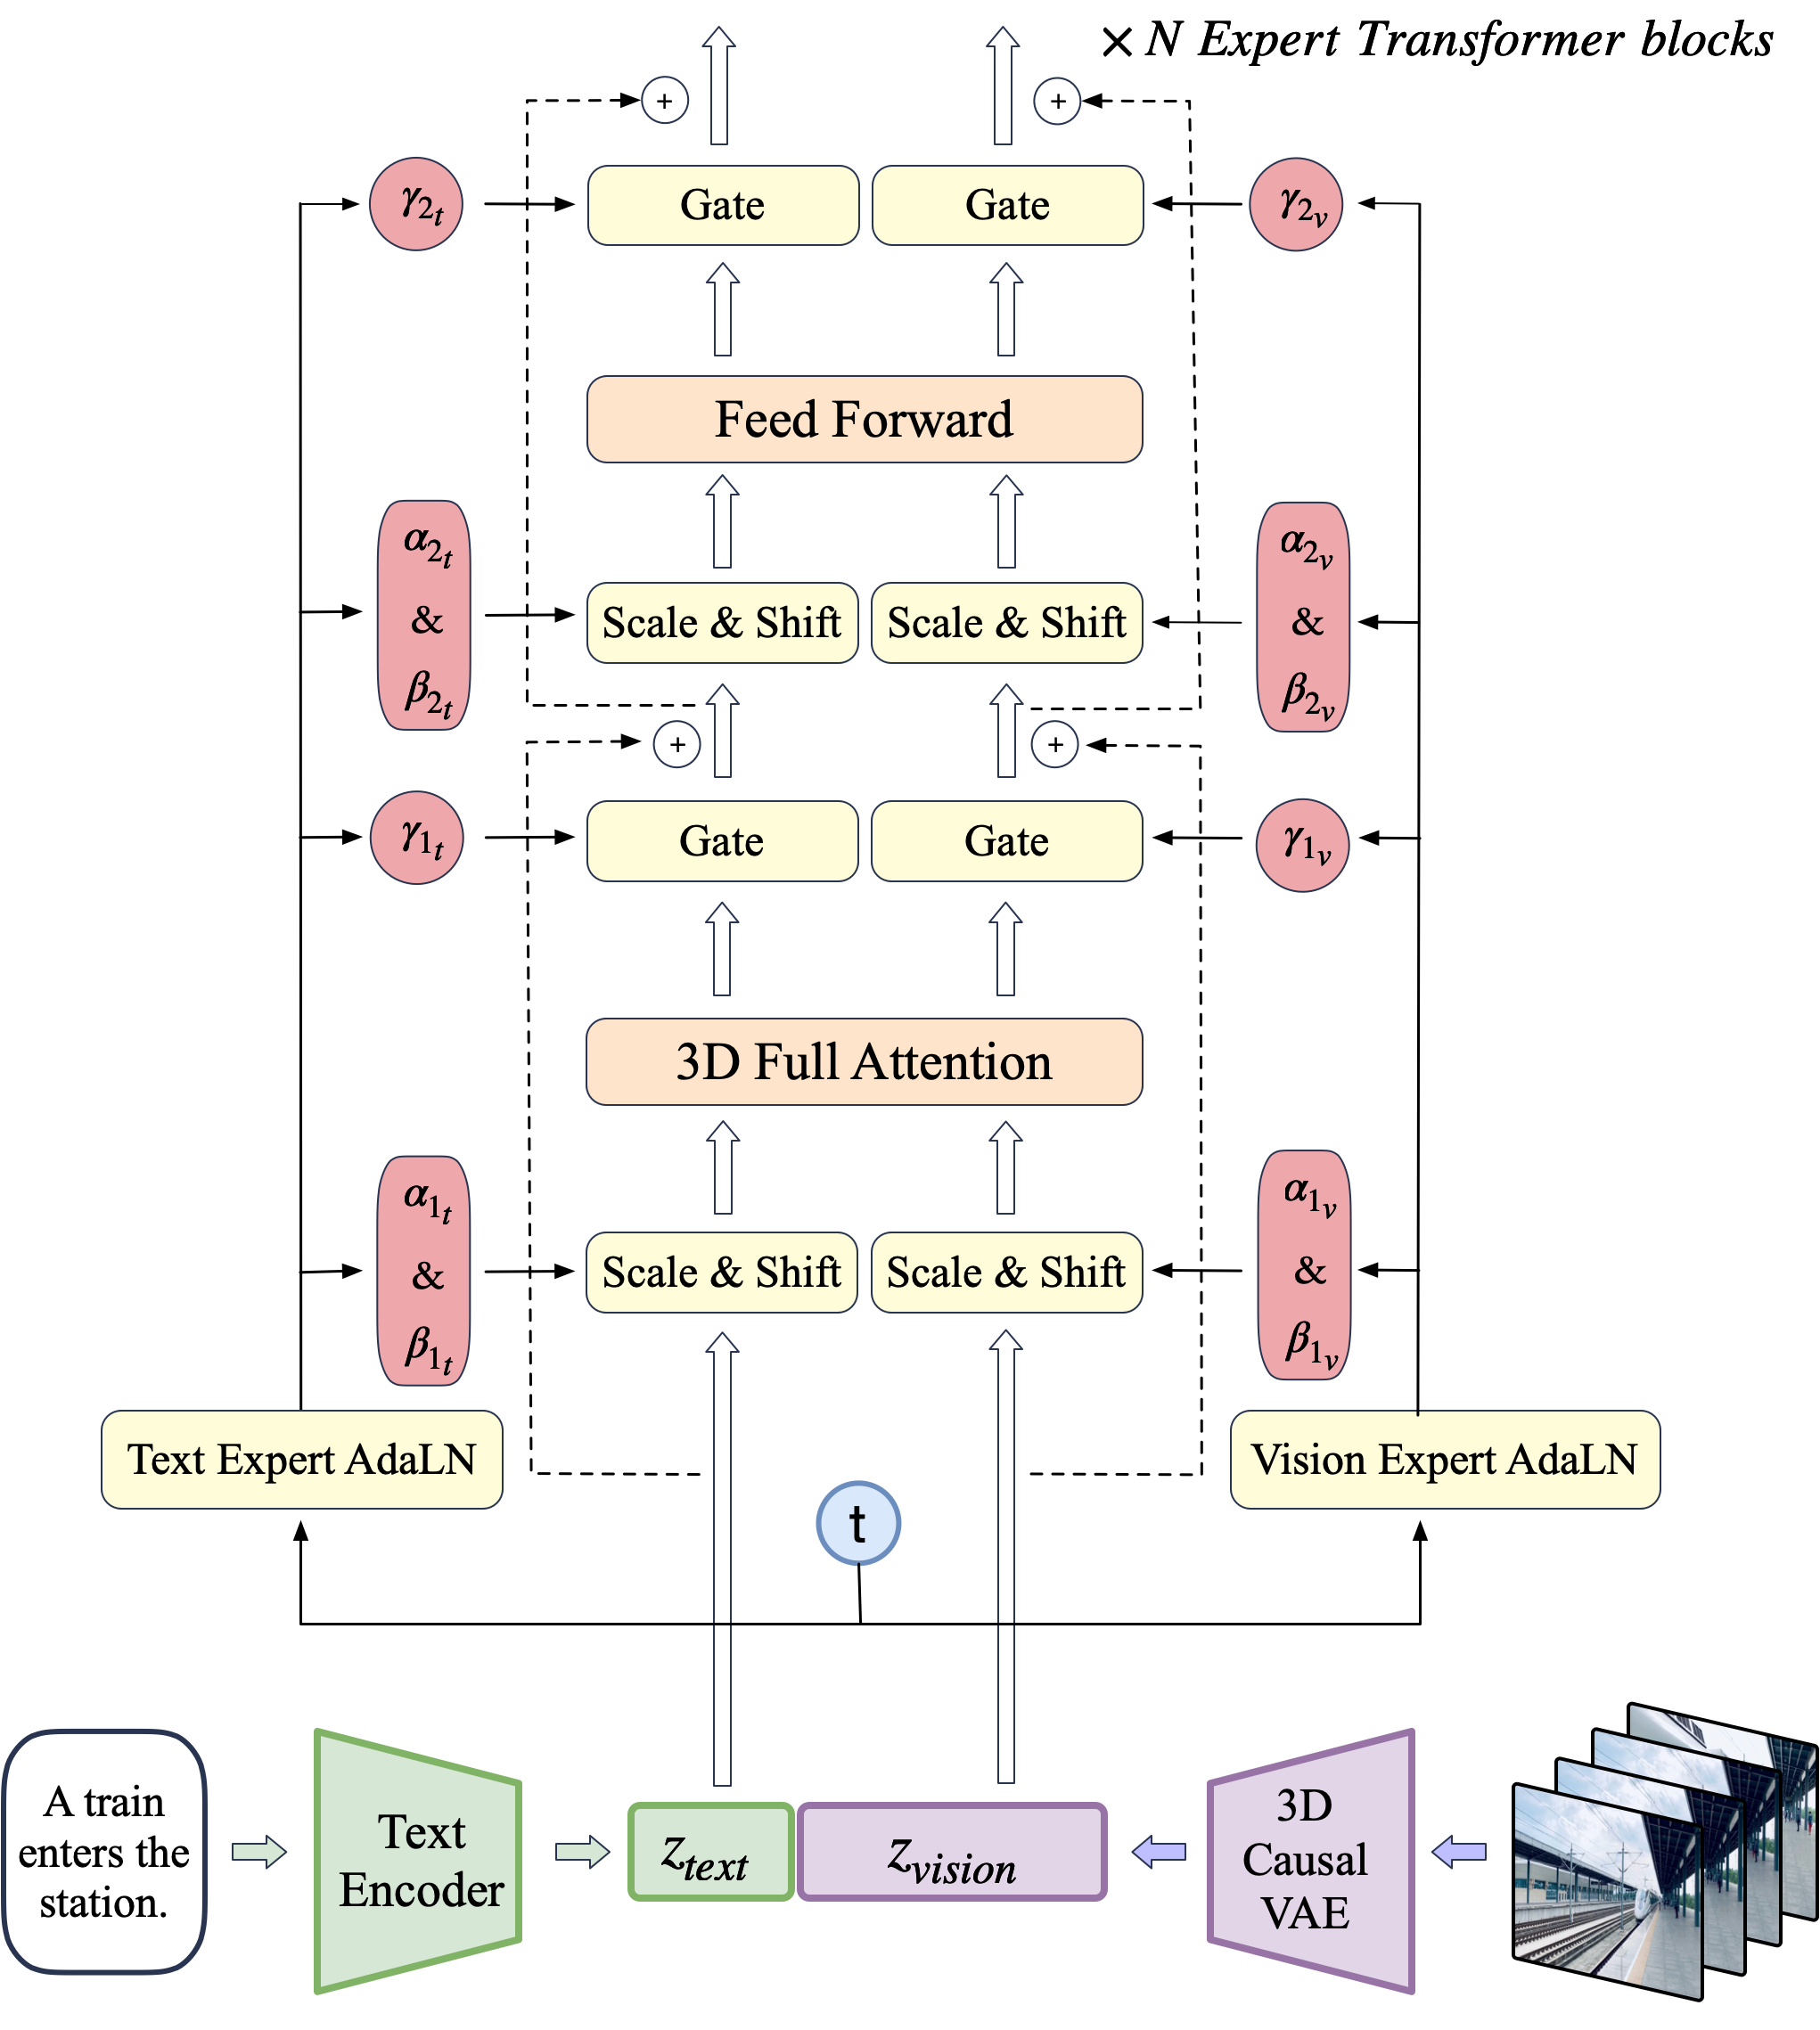
\includegraphics[width=0.7\linewidth]{images/transformer.png}
\end{center}
\caption{\textbf{Our model architecture.} }
\label{fig:model}
\end{figure}

\subsection{Expert Transformer}\label{sec:expert-transformer}

\paragraph{Patchify}
After being encoded into latent vectors of shape $T \times H \times W \times C$ by the 3D causal VAE, the video latents are patchified  along the spatial dimensions, resulting sequence $z_{\text{vision}}$ of length $T\cdot \frac{H}{p} \cdot \frac{W}{p}$. 
% VAE encodes the video into a latent vector of shape $T \times H \times W \times C$. Then we patchify the latent along the spatial dimensions, generating sequence $z_{vision}$ of length $T\cdot \frac{H}{p} \cdot \frac{W}{p}$. 
We do not patchify along the temporal dimension in order to enable joint training of images and videos.

\paragraph{3D-RoPE}
Rotary Position Embedding (RoPE)~\citep{su2024roformer} is a relative positional encoding that has been demonstrated to capture inter-token relationships effectively in LLMs, particularly excelling in modeling long sequences. To adapt to video data, we extend RoPE to 3D. 
Each latent in the video tensor can be represented by a 3D coordinate $(x, y, t)$.
We independently apply 1D-RoPE to each dimension of the coordinates, each occupies $3/8$, $3/8$, $2/8$ of the hidden states's channel. The resultsing encoding are then concatenate along the channel dimension to obtain the final 3D-RoPE encoding.

\paragraph{Expert Transformer Block}
We concatenate the embeddings of both text and video at the input stage to better align visual and semantic information. However, the feature spaces of these two modalities differ significantly, and their embeddings may even have different numerical scales. To better process them within the same sequence, we employ Expert Adaptive Layernorm to handle each modality independently.
As shown in Figure~\ref{fig:model}, following DiT~\citep{peebles2023scalable}, we use the timestep $t$ of the diffusion process as the input to the modulation module. 
Then, the Vision Expert Adaptive Layernorm and Text Expert Adaptive Layernorm independently apply this modulation mechanism to the vision hidden states and text hidden states respectively. This method promotes the alignment of feature spaces across two modalities while minimizing additional parameters.



\paragraph{3D Full Attention}
Previous works \citep{singer2022make, guo2023animatediff} often employ separated spatial and temporal attention to reduce computational complexity and facilitate fine-tuning from text-to-image models. However, as illustrated in Figure~\ref{fig:attention}, this separated attention approach requires extensive implicit transmission of visual information, significantly increasing the learning complexity and making it challenging to maintain the consistency of large-movement objects. Considering the great success of long-context training in LLMs and the efficiency of FlashAttention, we propose a 3D text-video hybrid attention mechanism. This mechanism not only achieves better results but can also be easily adapted to various parallel acceleration methods. 


\begin{wrapfigure}{r}{0.5\textwidth}
\centering
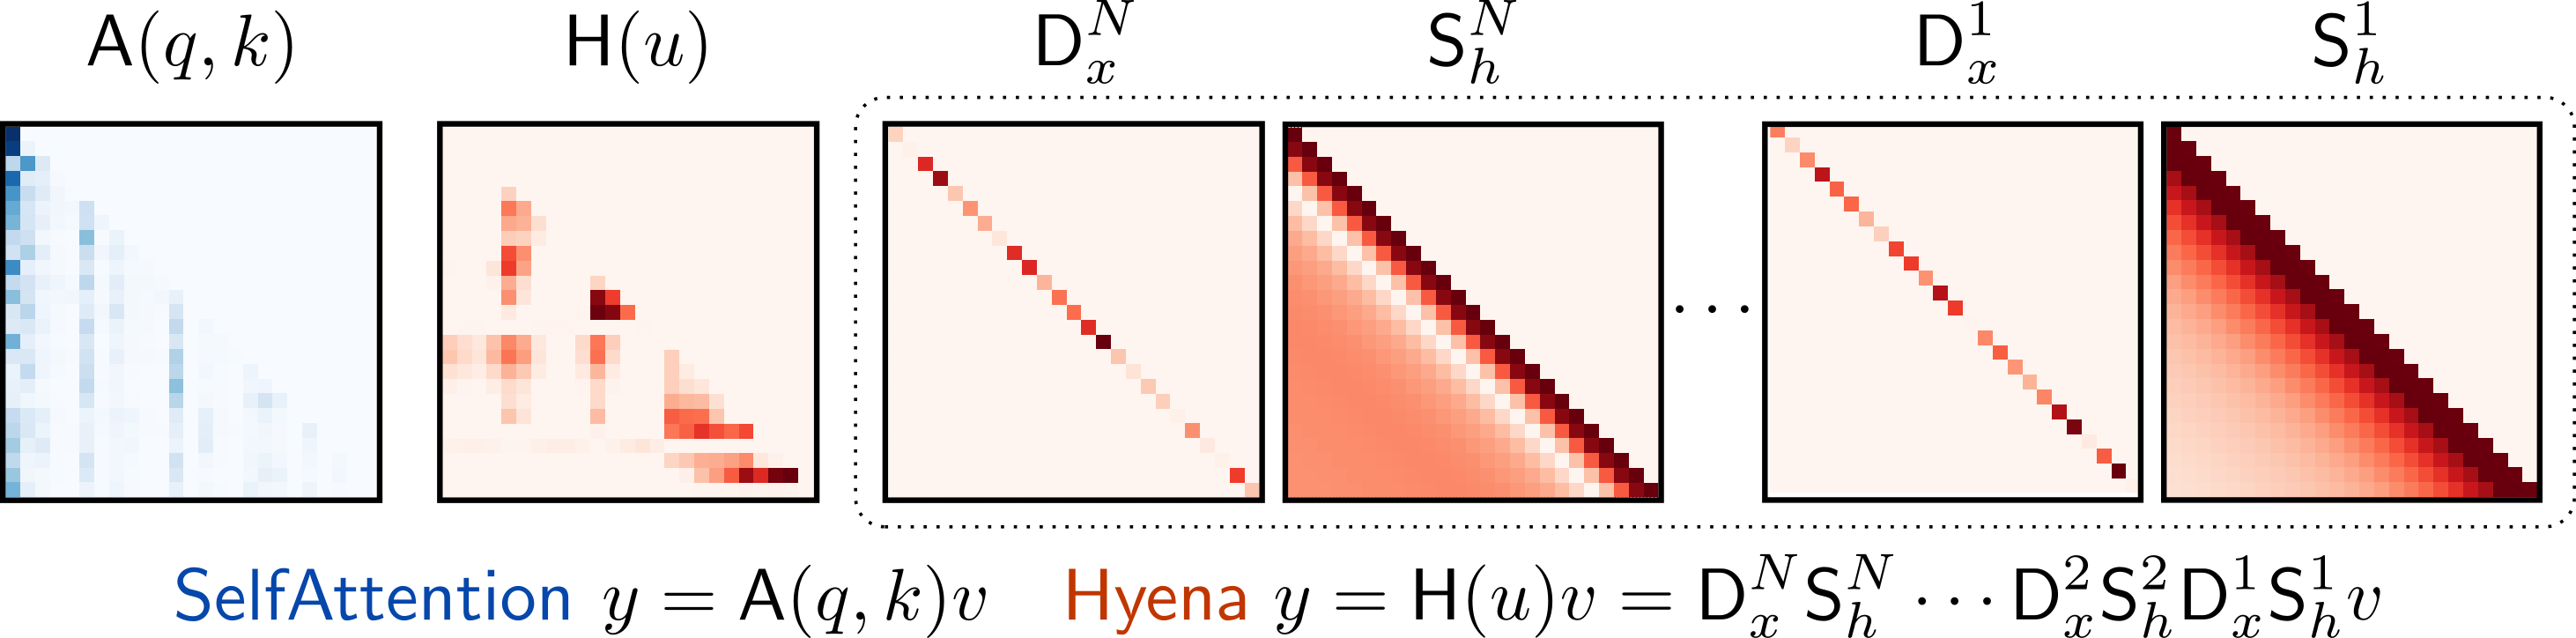
\includegraphics[width=\linewidth]{images/attention.png}
\caption{The separated spatial and temporal attention makes it challenging to  handle the large motion between adjacent frames. In the figure, the head of the person in frame $i+1$ cannot directly attend to the head in the frame $i$. Instead, visual information can only be implicitly transmitted through other background patches. This can lead to inconsistency issues in the generated videos.}
\label{fig:attention}
\vspace{-10mm}
\end{wrapfigure}





\section{Experiment configurations}
\label{sec:config}
\subsection{Datasets}
We trained and tested Apollo on the combined MUSDB18-HQ \cite{rafii2019musdb18} and MoisesDB \cite{pereira2023moisesdb} datasets. By integrating these two datasets, we leveraged their rich diversity and comprehensive musical resources to evaluate Apollo's restoration performance across different music genres more thoroughly. During the data preprocessing stage, inspired by music separation techniques \cite{uhlich2024sound,li2024subnetwork}, we employed a Source Activity Detector (SAD) to remove silent regions from the tracks, retaining only the significant portions for training. Throughout training, we implemented real-time data augmentation by randomly mixing tracks from different songs. Specifically, we randomly selected between 1 and 8 stems from 11 available tracks and extracted 3-second clips from each selected stem. These clips were then randomly scaled in energy within a range of [-10, 10] dB relative to their original levels. All selected stem clips were summed together to generate simulated music. Subsequently, we simulated dynamic bitrate scenarios by applying MP3 codecs with bitrates of [24000, 32000, 48000, 64000, 96000, 128000] to generate the compressed music. To ensure all samples were on the same scale, we rescaled both the target audio and the encoded audio based on the maximum absolute value.

\subsection{Hyperparameters}
For the proposed Apollo model, the Short-Time Fourier Transform (STFT) window length was set to 20 ms with a hop size of 10 ms, using a Hanning window. The bandwidth for frequency band segmentation was set to 160 Hz, and the feature dimension $N$ was set to 256. The Band Sequence modeling module was stacked $B = 6$ times. In the discriminator network, the STFT window sizes were configured with a multi-scale setup, including $[32, 64, 128, 256, 512, 1024, 2048]$. For the optimizer, both the generator and discriminator utilize the AdamW optimizer \cite{loshchilov2017decoupled}. The generator's initial learning rate was set to 0.001, with a weight decay of 0.01, while the discriminator's initial learning rate was set to 0.0001, with the same weight decay of 0.01. The learning rate decayed by 0.98 every two epochs, and gradient clipping with a maximum norm of 5 was employed to prevent gradient explosion. Additionally, we implemented an early stopping mechanism to prevent overfitting: training was terminated if the validation loss did not decrease for 20 consecutive epochs. All models were trained on 8 Nvidia RTX 4090 GPUs.

\subsection{Evaluation metrics}
In all experiments, we used the Scale-Invariant Signal-to-Noise Ratio (SI-SNR) \cite{le2019sdr}, Signal-to-Distortion Ratio (SDR) \cite{vincent2006performance}, and Virtual Speech Quality Objective Listener (VISQOL) \cite{hines2015visqol} to evaluate the quality of the reconstructed audio. To assess the model's efficiency, we reported the time consumption per second of audio processed by Apollo and SR-GAN (Real-Time Factor, RTF). RTF is calculated by processing 1-second audio tracks sampled at 44.1 kHz on both CPU and GPU, and the average value is taken after running 1000 iterations. Additionally, we measured the model size by reporting the number of parameters using the open-source tool PyTorch-OpCounter\footnote{\url{https://github.com/Lyken17/pytorch-OpCounter}}.

\section{Results}
\label{sec:result}
\begin{table*}
\small
\centering
\def\arraystretch{1.35}
\begin{tabular}{|l|l|l|l|l|l|}
\hline
      Dimension      & Test & GPT3.5 & GPT4 & Claudev1.3 & Human                         \\ \hline
\multirow{5}{*}{Fluency} & Understandability \& Coherence                                                     &  15.0      & 30.0     &      55.0     &  \textbf{90.0}     \\ \cline{2-6}
 & Narrative Pacing                                                                   &  10.0      &   50.0   &       70.0    &   \textbf{90.0}   \\ \cline{2-6}
 & Scene vs Exposition                                                                &  10.0      &   60.0   &     65.0      &  \textbf{85.0}     \\ \cline{2-6}
 & \begin{tabular}[c]{@{}l@{}}Literary Devices \& Language Proficiency\end{tabular} &   5.0     &   40.0   &     15.0      & \textbf{80.0}      \\ \cline{2-6}
 & Narrative Ending                                                                   & 10.0       & 20.0     &      45.0     &  \textbf{85.0}     \\ \hline\hline
\multirow{3}{*}{Flexibility} & Emotional Flexibility                                                              &   20.0     &  25.0    &    55.0       &  \textbf{90.0}    \\ \cline{2-6}
& Perspective \& Voice Flexibility                                                   &  10.0     &   20.0   &     25.0      &  \textbf{70.0}     \\ \cline{2-6}
& Structural Flexibility                                                             &  15.0      &  30.0    &    35.0       & \textbf{90.0}     \\ \hline\hline
\multirow{3}{*}{Originality} & Originality in Form \& Structure                                                   & 0.0       &   15.0   &     0.0      &  \textbf{60.0}     \\ \cline{2-6}
& Originality in Thought                                                             &   5.0     &   60.0   &     35.0      &  \textbf{90.0}     \\ \cline{2-6}
& Originality in Theme \& Content                                                    &  0.0      &  30.0    &     10.0      &  \textbf{85.0}     \\ \hline\hline
\multirow{3}{*}{Elaboration} &  World Building \& Setting                                                          &   15.0     &   35.0   &    65.0       &  \textbf{90.0}    \\ \cline{2-6}
& Character Development                                                              &   10.0     &  20.0   &  25.0        &  \textbf{75.0}    \\ \cline{2-6}
& Rhetorical Complexity                                                              &    5.0    &  10.0    &    10.0       &  \textbf{90.0}    \\ \hline
\end{tabular}
\vspace{2ex}
\caption{\label{absolutehumaneval}\textbf{Absolute Evaluation}: Average passing rate on individual creativity test obtained from 8 creative writing experts across all stories in our test set authored by GPT3.5,GPT4,Claude and Humans}

\begin{tabular}{|l|l|l|l|l|}
\hline
                                                                               & GPT3.5 & GPT4 & Claudev1.3 & Human \\ \hline
\begin{tabular}[c]{@{}l@{}}Relative Ranking Based on Preference\end{tabular} & 3.45   & 3.0  & 2.35       & 1.2   \\ \hline
\end{tabular}
\vspace{2ex}
\caption{\label{relativehumaneval} \textbf{Relative Evaluation}:Average ranking provided by 8 creative writing experts based on their subjective preference across all stories in our test set authored by GPT3.5,GPT4,Claude and Humans}
\end{table*}

\section{Conclusion}
\label{sec:conclusion}

Hyperbolic embeddings embed hierarchical information with high
fidelity and few dimensions. We explored the limits of this approach
by describing scalable, high quality algorithms. We hope the
techniques here encourage more follow-on work on the exciting
techniques of \citet{fb, ucl}. As future work, we hope to explore how
hyperbolic embeddings can be most effectively incorporated into downstream
tasks and applications.


\bibliographystyle{IEEEtran}
\bibliography{refs}

\end{document}
